\documentclass{article}
\usepackage[backend=bibtex]{biblatex}
\usepackage[margin=1in]{geometry}
\usepackage{amsmath}
\usepackage{amssymb}

\usepackage{graphicx}
\usepackage[space]{grffile} %for filepaths with spaces

\bibliography{../references} % the name of your .bib bibliography file, without the file extension

% some helpful math commands I like to define
\newcommand{\vect}[1]{\ensuremath{\mathbf{#1}}}
\newcommand{\mat}[1]{\ensuremath{\mathbf{#1}}}
\newcommand{\transpose}{\ensuremath{\mathsf{T}}}
\newcommand{\of}[1]{\ensuremath{\left(#1\right)}}

%define degree symbol:
\newcommand{\degree}{\ensuremath{^\circ}}
\newcommand{\fr}[1]{$#1^+$} %command to write a reference frame
\newcommand{\br}[2]{[#1]_{#2}} %bracket operator with subscript
\newcommand{\tvect}[3]{\begin{bmatrix}#1\\#2\\#3\end{bmatrix}}% 3 x 1 vector
\newcommand{\tvecth}[3]{\begin{bmatrix}#1&#2&#3\end{bmatrix}}% 1 x 3 vector
\newcommand{\B}[1]{\textbf{#1}} %bold for regular vectors
\newcommand{\U}[1]{\hat{\textbf{#1}}} %hats and bold for unit vectors
\newcommand{\BG}[1]{{\bm #1}}           % for vectors using greek letters
\newcommand{\ddt}[1]{\frac{d#1}{dt}} %for time derivatives
\newcommand{\ddarg}[2]{\frac{d#1}{d#2}} % for general derivatives
\newcommand{\pparg}[2]{\frac{\partial#1}{\partial#2}} % for general derivatives
\newcommand{\kron}{\otimes} %redefines \kron to produce kronecker product symbol, for convenience

% document information
\title{Pathfinder Status Update August 23 2014}
\author{Tim Woodbury \\ \normalsize{Texas A\&M University}}
\date{\today} % or put in a fixed date (e.g. 12 June 2014) if you want it to stay put

% outline
% intro
% research work
%	Cooperative localization
%		Range & bearing
%		Bearing only
%		Bearing only w/ IMU sharing
% REEF work
%	Optitrack management
%		Smoothing
%		Time synching
%	drag characterization
%		Ardrone
%		3DR Quadrotor
%	sensor char & estimator evaluation

\begin{document}
\maketitle

\section{Introduction}

Activities are summarized in two sections. The first details university research, which has focused on establishing a framework for conducting cooperative estimation simulations. The second details hardware-related work for the quadrotor lab at the REEF.

\section{University research}

Cooperative estimation is a broad topic of collective interest to the associated institutions. The cooperative estimation problem as defined here refers to a scenario with at least two vehicles who share some set of measurement data to improve estimator accuracy. A restricted subproblem with two planar agents has been considered. Agents have typical inertial measurement unit (IMU) measurements of acceleration and angular velocity. Agents measure range and bearing to one another, which enables agents to exchange and exploit measurements without coupling their state estimates. Agents also measure bearing and sometimes range to features in the workspace. Initial evaluation was performed using known features. Three subproblems have been considered: (1) Agents measure and share range and bearing to features; (2) Agents measure and share feature bearing only; (3) Agents measure and share feature bearing, and also share IMU data. In the first two cases, agents estimate only their own state, and in the third case states are added to account for the other agent's relative position and heading, and absolute velocity. Preliminary results validate the basic approach. In the future, this approach will be extended to 3D problems with potentially unknown features.

\section{REEF work}

Work at the REEF has had three main focus areas: (1) processing of Optitrack inertial measurement data and vehicle onboard logs; (2) Drag characterization of the AR.drone and 3DR Quadrotor platforms; (3) Characterization of vehicle sensors and estimator tuning.

\subsection{Optitrack data}

The Optitrack motion capture system uses retro-reflective markers to detect and track rigid body rotation and translation. The system is not intended for active control of the quadrotor plants; it provides high-accuracy inertial measurements, and has been used to provide truth data for characterizing the quadrotor dynamics and sensors. Data are recorded at 120 Hz and measurement error is nominally on the order of millimeters. Incorporation of Optitrack into the Pathfinder project can be summarized in two sections: (1) direct processing of Optitrack data to produce usable vehicle velocity and acceleration-level histories; (2) joint processing of Optitrack and onboard data.

Low-pass filters were implemented to produce smooth vehicle velocity and acceleration-level histories. Differencing position and attitude measurements provides noisy histories of the body translational and angular velocities. During relatively slow flying, the differenced histories may be smooth enough to be used without further postprocessing; however, more rapid movement intermittently produces discontinuities in the differenced histories. Digital Butterworth filters were implemented to provide smoother trajectories in the absence of model-based estimation for a given rigid body, allowing direct comparison of motion capture and onboard state histories in postprocessing. Acceleration-level histories can be generated by a subsequent differentiation of the velocity histories, but obtaining smooth histories is not always possible. Optitrack-derived acceleration histories are generally smooth enough to at least permit qualitative comparison against vehicle data.

At present, Optitrack and vehicle sensors are logged independently and use separate time scales. Multiple methods for synchronizing the two time scales in postprocessing have been implemented. Good results have been achieved by examining variables recorded in both time scales and computing the time shift from their 1-D phase correlation\footnote{See section ``Phase correlation time sync'' at  \url{https://wiki.antcenter.net/display/PATH/Record+and+sync+motion+capture+and+autopilot+histories?src=search}}. Estimating the time shift in this way has generally proved reliable and, after interpolating the higher-resolution motion capture data, enables direct comparison against onboard data. This comparison has been extremely useful for vehicle drag characterization, sensor characterization, and estimator evaluation.

\subsection{Drag coefficient}
\label{sec:drag}

Recent literature shows that IMU-based estimation accuracy can be improved by inclusion of linear drag terms\cite{macdonald2014}. Experimental testing of this estimator has indicated that estimation accuracy is highly sensitive to the value of the drag parameter. A fusion of the motion capture and vehicle sensor data was used to characterize the AR.drone and 3DR quadrotor platforms, and is summarized here.

The governing equations for velocities $u$ and $v$ are written in terms of the vehicle angular rates $p,q,r$, vertical velocity $w$, gravity magnitude $g$, roll and pitch angles $\phi$ and $\theta$, and drag forces $F_{di}$ and $F_{dj}$:

\begin{align}
\dot{u} = -g\sin{\theta} + vr-wq - \frac{F_{di}}{m} \label{eq:govu} \\
\dot{v} = g\sin{\phi}\cos{\theta} + wp-ur - \frac{F_{dj}}{m} \label{eq:govv}
\end{align}

The drag forces are assumed to have the following forms:

\begin{align}
F_{di} = \mu u\\
F_{dj} = \mu v
\end{align}

The term $\mu$ is an unknown, assumed constant drag coefficient to be estimated from flight data. Note that the Eqs. \ref{eq:govu} and \ref{eq:govv} can be written in terms of the associated vehicle body-frame accelerations $a_1$ and $a_2$:

\begin{align}
a_1 = -g\sin{\theta} - \frac{\mu}{m}u\\
a_2 = g\sin{\phi}\cos{\theta} - \frac{\mu}{m}v
\end{align}

In a vector form, the preceding expression may be written in terms of the acceleration vector \B{a}, the normalized gravity force vector $g\U{n}_3$, and the drag force normalized by mass $\B{f}_d$:

\begin{equation}
\B{a} = g\U{n}_3 - \B{f}_d
\end{equation}

At this point, it is worth recalling that vehicle accelerometer measurements $\tilde{\B{a}}$ are modelled as a function of the true accelerations, a Gaussian noise term $\B{v}$, and the gravity vector:

\begin{equation}
\tilde{\B{a}} = \B{a} - g\U{n}_3 + \B{v}
\end{equation}

This leads to the following relationship between the accelerometer measurements and the normalized drag force:

\begin{equation}
\tilde{\B{a}} = -\B{f}_d + \B{v} = -\frac{\mu}{m}\begin{bmatrix}
u\\v
\end{bmatrix} + \B{v}
\end{equation}

Measurements of acceleration are available from the vehicle accelerometer and from twice-differenced motion capture time histories. Note that the raw accelerometer data can be directly correlated with the drag force, but the acceleration histories from motion capture must account for the gravity component, which couples the acceleration history with attitude. Velocity measurements are provided from the optic flow sensor on the vehicle and from once-differenced motion capture histories. Linear least-squares fits for $\mu$ were computed using combinations of measurements from the different sources. Consistent results that led to good estimator performance were attained using vehicle accelerometer data with velocity histories interpolated from the motion capture data.

As has been mentioned previously, motion capture data experiences intermittent spikes in the noise level, which manifest as pulse discontinuities in the motion capture velocity histories. To account for these spikes, the data were segmented such that no spikes are contained in any given time segment. Best fits for $\mu/m$ were fit to each segment individually and to all segments at once, to check for agreement. By comparing the parameter fits between different segments, confidence metrics were obtained.

Parameter identification is theoretically independent of how the vehicle is flown, as long as the accelerometer signal-to-noise ratio (SNR) is sufficiently large. In test flights, the vehicles were flown under manual control. The vehicle 1 and 2 axes were alternately excited by flying at the maximum speeds comfortable for the operator along each direction.

Drag characterization has been performed for the AR.drone in two configurations: (1) standard configuration with PX4 autopilot and PX4FLOW optic flow sensor; (2) configuration with ODROID onboard computer. Table \ref{tab:nomDrag} summarizes the identified models for the two AR.drone configurations and the 3DR quadrotor. In this table, $\Delta(\mu/m)_{95\%}$ indicates a 95\% confidence interval for the drag ratio $\mu/m$. This confidence interval is computed by assuming that the drag coefficients identified in each time segment represent independent samples of a single random variable, and should not be interpreted in a statistically rigorous fashion. However, $\Delta(\mu/m)_{95\%}$ is a reasonable metric of the relative agreement between the parameters fit to different time segments. The number of time segments used to obtain each parameter is given by $n$.

Despite a comparatively small number of flight segments, the 3DR drag estimate has the tightest confidence interval. This is thought to be a product of two factors. (1) The 3DR quadrotor has much larger rotors than the AR.drone. Since the drag term in intended to incorporate rotor drag, it is possible that the drag term has a greater effect on the 3DR dynamics and correlates more strongly with the measured accelerations. (2) the lighter AR.drone experiences notable structural vibrations, which manifest as periodic signals in the accelerometer histories. This phenomenon might lead to greater apparent variance in IMU measurements, which could make identified drag ratios more variable. The AR.drone was particularly difficult to characterize, as can be seen by the 11 flights with the ODROID required to obtain a confidence interval on the order of the 3DR confidence interval.

\begin{table}[tb!]
\centering
\begin{tabular}{|c|c|c|c|c|c|}
\hline
Platform & $\mu/m$ & $\Delta(\mu/m)_{95\%}$ & $\mu$ & $m$ (kg) & $n$ \\
\hline
AR.drone & 0.4 & 0.16 & 0.15 & 0.36 & 6\\
\hline
AR.drone with ODROID & 0.40 & 0.049 & 0.24 & 0.598 & 11\\
\hline
3DR Quadrotor & 0.29 & 0.031 & 0.35 & 1.21 & 4 \\
\hline
\end{tabular}
\caption{Comparison of identified drag parameters for each vehicle. $n$ is the number of time segments used for identification.}
\label{tab:nomDrag}
\end{table}

\subsection{Sensor characterization and estimator testing}

A primary objective of this summer's work has been implementation of a more sophisticated onboard attitude and velocity estimator. Reasonably accurate values of the various sensor noise variances are needed for accurate estimation. Some values, such as vehicle body-frame accelerations, are difficult to characterize due to low accuracy in the associated motion capture time histories. Initial values were estimated from vehicle data, and tuned once the estimator was implemented to improve estimation accuracy.

Tests were performed to characterize the vehicle accelerometers, gyroscopes, sonar rangefinder, and optic flow sensor. In principle, each sensor should be straightforwardly characterized by flying the vehicle while recording onboard and motion capture data, computing the error between motion capture and onboard measurements, and determining appropriate standard deviations. For position histories, motion capture data are very reliable and can readily be treated as ``truth'' values. The velocity-level and particularly the acceleration-level histories are generally much noisier and less smooth, making direct comparison of onboard and motion capture histories problematic and introducing spurious noise.

Knowing that the estimator would be evaluated initially in simulation using flight data, where the noise parameters could readily be tuned, initial noise levels for most sensors were generated by initializing the vehicle on the ground and collecting 15 seconds of data, taking off, engaging the autopilot's built-in ``easy mode'' position controller for approximately 10 seconds, then landing and collecting another 15 seconds of data. The primary objective of this exercise was to compare vehicle measurements before and after takeoff and landing. However, for the accelerometers in particular, the signal magnitude during hovering flight should be low enough that the standard error of the raw measurements is a conservative approximation of the sensor standard deviation. The following sections summarize the initial findings for the vehicle IMU, the procedure and results for the optic flow sensor and sonar, and the updated values that were eventually used in the estimator in hardware.

\subsubsection{IMU variance}

Table \ref{tab:imustd} summarizes the initial values identified as the IMU noise characteristics. These values were expected to be quite approximate. Standard errors of the sensor measurements were computed for the two at-rest segments and the one hovering segment of each of two characterization flights. The presented IMU characteristics were conservatively taken as 150\% of the largest standard error identified from any data collection segment.

\begin{table}
\centering
\begin{tabular}{|c|c|}
\hline
Sensor & Standard deviation \\
\hline
Accelerometer ($\mathrm{m/s^2}$) & 0.83 \\
\hline
Gyroscope (rad/s) & 0.12 \\
\hline
\end{tabular}
\caption{Initial identified values of IMU standard deviations.}
\label{tab:imustd}
\end{table}

\subsubsection{Optic flow sensor and sonar rangefinder}

The optic flow sensor consists of a 752 $\times$ 480 resolution imager, a three-axis gyroscope, and a sonar rangefinder. Operation is detailed in Ref. \cite{honegger2013} and briefly summarized here. Images are downsampled and the raw pixel shift between the current and previous images is computed by an onboard ARM microcontroller. The gyroscope is used to compensate for the rotation of the imager relative to the scene, and the rangefinder is used to convert the raw pixel shift into a linear distance travelled. Due to the algorithm used to determine pixel shift at a fast rate, the sensor is only rated to work at up to a 1 m/s speed per meter of altitude, and the stock sonar limits the maximum effective altitude to approximately 5 m. The sonar is very accurate for ranges between its minimum of 30 cm and its maximum. However, it intermittently produces false returns that appear as single-point spikes in the sensor history.

The optic flow sensor has proven challenging to characterize. After much investigation, comparison flights on the AR.drone and 3DR quadrotors indicated that the SNR profile was much more favorable for the flow sensor on the 3DR platform than on the AR.drone. (Comparative tests were conducted using the same flow sensor, moved between the two platforms.) Different structural vibration profiles on the two platforms may explanation this discrepancy. On the AR.drone, it was observed that the SNR would sometimes improve substantially when the vehicle velocity was nonzero. The flow sensor was profiled by manually selecting flight data where the flow variance appeared to be low. 

Two flights were conducted under manual control, in which the vehicle was flown at different altitudes to investigate the influence of altitude on flow residuals. Errors were binned based on altitude rounded to the nearest 0.125 m, and the variance of each bin was computed. Results for two flights are shown in Fig. \ref{fig:resids_v_alt_bins}. A proposed model is also plotted. As a function of altitude, $h$, the proposed model gives the standard deviation of the flow sensor x-y measurements $\sigma(h)$ for each axis as:

\begin{equation}
\sigma(h) = \begin{cases}
0.4 \ \mathrm{m/s}, & \text{if $h \leq 0.5 $ m} \\
(0.68h + .06) \ \mathrm{m/s}, & \text{if $ .5 < h \leq 1.75 $ m} \\
1.25 \ \mathrm{m/s}, & \text{if $h > 1.75 $ m}
\end{cases}
\label{eq:sigmamodel}
\end{equation}

For simulation purposes, Eq. \ref{eq:sigmamodel} is identified as a tentative optic flow sensor model. The maximum expected standard deviation of 1.25 m/s is identified as an initial value for the estimator. Comparison of the 3$\sigma$ bounds given by Eq. \ref{eq:sigmamodel} with the flow sensor residuals for the full flights (not shown) indicates that the 3$\sigma$ bounds qualitatively encompass the typical residuals in a conservative fashion.

\begin{figure}[tb!]
\centering
\begin{minipage}{0.49\textwidth}
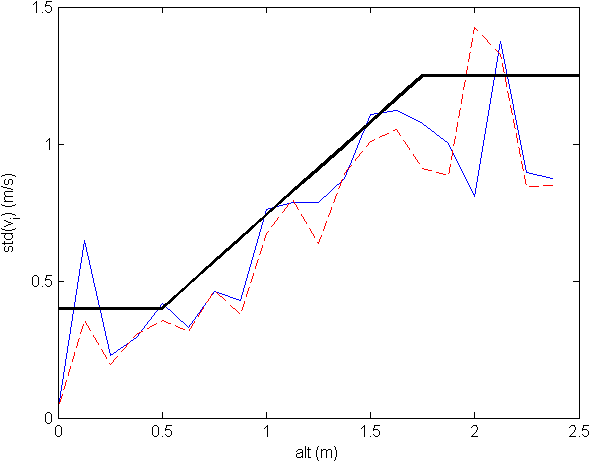
\includegraphics[width=\textwidth]{../../sensor characterization/flow figures/resids_v_alt1_bins.png}
\end{minipage}
\begin{minipage}{0.49\textwidth}
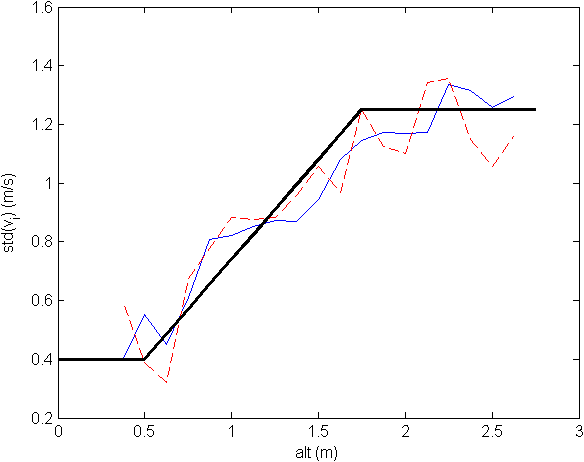
\includegraphics[width=\textwidth]{../../sensor characterization/flow figures/resids_v_alt2_bins.png}
\end{minipage}
\caption{Variance of binned errors for the two flights. Solid lines indicate the sensor x-axis error, dashed lines indicate the y-axis error. The black line indicates the suggested fit and is the same for both figures.}
\label{fig:resids_v_alt_bins}
\end{figure}

The flow sensor is characterized by nominally centimeter-accurate results with unpredictable single-point spikes in the time history. Fig. \ref {fig:movingflyingalt} is representative, in that motion capture and sonar readings are essentially identical except for a handful of false returns from the sonar. Table \ref{tab:altErrs} shows the mean and standard error from the two test flights, along with the proportion of sonar returns that were found to be false returns. The proportion of false returns can be quite high, but the accuracy is very good otherwise. A conservative standard deviation of 8.3 cm was identified and was used throughout the subsequent estimator development. Outlier rejection was performed by excluding measurements less than the minimum sensitivity and greater than 4 m in altitude, as well as any measurement that differed from the prior one by 0.5 m. (The latter criterion should be considered in light of the nominal sample rate of 250 Hz.)

Fig. \ref{fig:movingflyingalthist} shows the histogram of sonar errors from one flight after outliers are removed, along with a normal distribution best-fit. The histogram bins are concentrated at the center of the distribution, meaning that fewer errors far from 0 were measured than a normal distribution would imply. It is assumed that this fit is conservative compared to the actual sensor performance.

\begin{figure}[tb!]
\centering
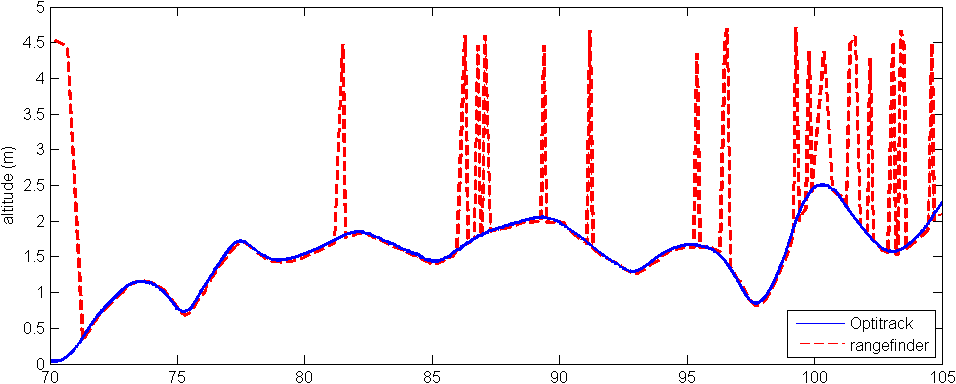
\includegraphics[width=0.8\textwidth]{../../sensor characterization/moving_flying_alt.png}
\caption{Sonar range measurements and motion capture altitude during flight.}
\label{fig:movingflyingalt}
\end{figure}

\begin{table}
\centering
\begin{tabular}{c|c|c|c}
Segment & Mean altitude error (m) & Standard error (m)& Fraction of bad returns\\
1 & 0.035 & 0.055 & 0.20\\
2 & 0.026 & 0.031 & 0.085\\
\end{tabular}
\caption{Summary of in-flight errors from ultrasonic rangefinder.}
\label{tab:altErrs}
\end{table}

\begin{figure}[tb!]
\centering
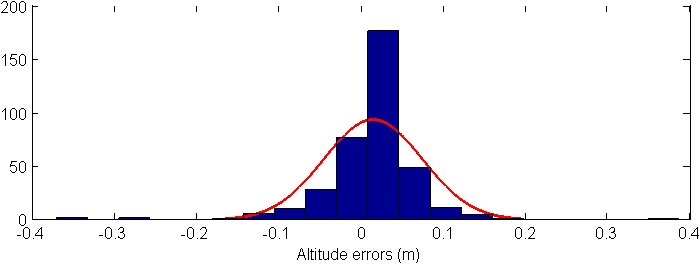
\includegraphics[width=0.8\textwidth]{../../sensor characterization/moving_flying_alt_hist.png}
\caption{Histogram of ultrasonic rangefinder measurements after removing outliers.}
\label{fig:movingflyingalthist}
\end{figure}

\subsubsection{Estimator testing}

Subsequently, the estimator was evaluated in MATLAB and implemented on the PX4 hardware. My association with the estimator implementation has primarily been in evaluating the estimates compared to the motion capture velocity and attitude histories. Additionally, updated drag parameters were identified as a result of estimator performance and were found to enhance accuracy significantly.

Simulation results indicated that the form of the estimator implemented by the Pathfinder team should be more accurate than the one implemented in the default PX4 firmware. However, the initial hardware implementation on the AR.drone showed that the Pathfinder attitude estimates had noticeably larger standard errors. Notably, the initial implementation on the 3DR platform performed better than on the AR.drone, such that its standard errors were still larger than the stock estimator, but were typically within a fraction of a degree in roll and pitch. This was significant because the 3DR drag coefficient was obtained using the method of Sec. \ref{sec:drag}, while the AR.drone estimate was initially obtained using Observer-Kalman Filter Identification. When the AR.drone drag characterization was repeated using the approach of Sec. \ref{sec:drag}, its estimator performed similarly to the 3DR's.

Additional investigation in MATLAB revealed that the Pathfinder estimator performed better with larger accelerometer noise and lower gyroscope noise. It should be noted that the gyroscope values initially implemented were intended to capture additional error brought about by not estimating the IMU biases; however, this assumption also reduced estimation accuracy. By implementing new variance levels in the hardware implementation, the Pathfinder estimator achieved lower standard errors in attitude than the stock estimator. As expected, the Pathfinder estimates in that case did exhibit a significant bias that depended strongly on the IMU calibration. However, this experiment demonstrated in principle that the Pathfinder implementation was functionally correct. An objective for the near future is to extend the estimator to estimate IMU biases.

Fig. \ref{fig:attcmp} compares the Pathfinder estimator to the stock PX4 attitude estimator during aggressive pitch maneuvers. The Pathfinder estimator tracks qualitatively better for larger attitude deflections than the stock estimator does. Additionally, the standard errors relative to  capture data are slightly lower for the Pathfinder estimator (see Table \ref{tab:attcmp}). The values listed in Table \ref{tab:attcmp} were obtained from a single flight lasting about 1 minute, and are not presented as statistically singificant comparisons. The values are representative of performance observed over several flights, in which the standard error for the Pathfinder estimator was consistently smaller than for the PX4 estimator.

\begin{figure}[tb!]
\centering
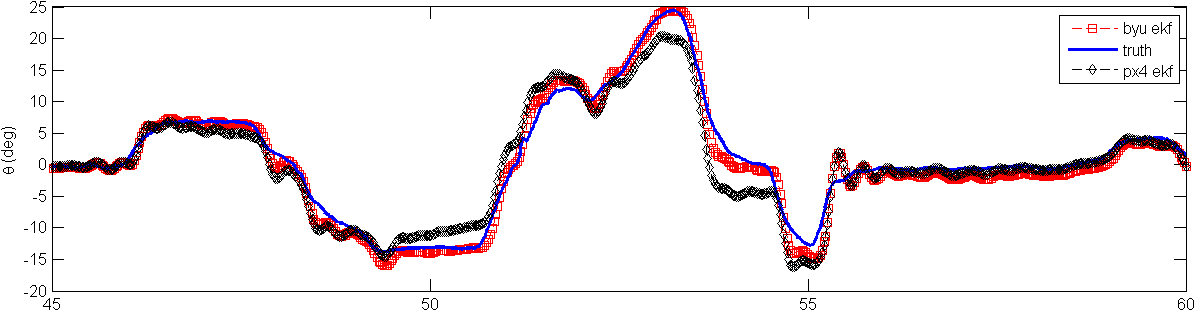
\includegraphics[width=0.9\textwidth]{../../sensor characterization/aug6_3dr_ekf_test1_pitch_cmp.png}
\caption{Comparison of Pathfinder, or BYU-style, EKF with PX4 stock attitude estimator during aggressive maneuvers of 3DR quadrotor.}
\label{fig:attcmp}
\end{figure}

\begin{table}[tb!]
\centering
\begin{tabular}{|c|c|c|}
\hline
Estimator & $S(\phi)$ (deg) & $S(\theta)$ (deg)\\
\hline
Pathfinder & 1.13 & 0.786\\
\hline
PX4 stock & 1.17 & 1.02\\
\hline
\end{tabular}
\caption{Comparison of attitude standard errors $S$ for the Pathfinder and PX4 estimators during one flight test.}
\label{tab:attcmp}
\end{table}

\printbibliography

\end{document}
